\begin{center}
	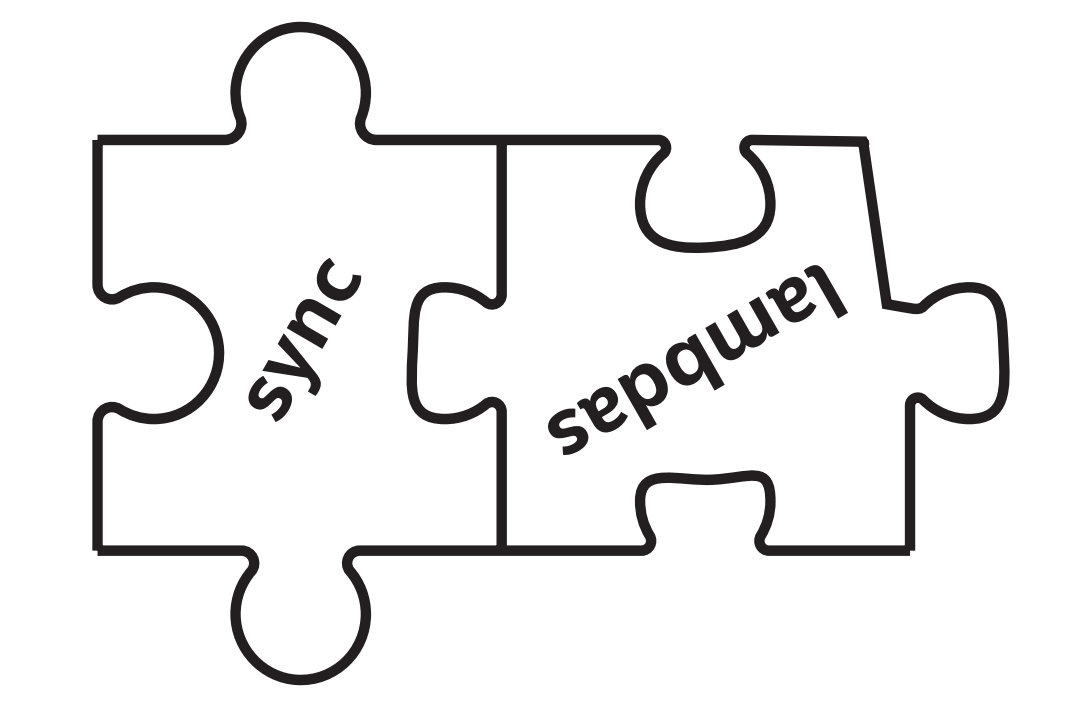
\includegraphics[width=0.5\textwidth]{content/chapter-10/images/1}
\end{center}

目前为止,代码示例使用C++ Lambda表达式表示内核。Lambda表达式是表示内核的一种简洁方便的方法,但不是SYCL中表示内核的唯一方法。本章中,我们将探索各种详细定义内核的方法,从而选择最适合C++编码需求的内核形式。\par

本章解释和比较了三种表示内核的方法:\par

\begin{itemize}
	\item Lambda表达式
	\item 命名函数对象(functor)
	\item 与其他语言或API创建的内核的互动性
\end{itemize}

本章讨论了如何显式地操作程序对象中的内核,控制何时以及如何编译内核。\par




